\documentclass[24pt]{beamer}

\usepackage{graphicx}
\usepackage{titlesec}
\usepackage{listings} % For inserting code
\usepackage[margin=0.5in]{geometry} % For adjusting the margin size
\usepackage{wrapfig}
\usepackage{mathtools}
\usepackage{multicol}

\usetheme{metropolis}           % Use metropolis theme
\title{G54SOD}
\subtitle{Developing a Smart Campus}
\date{Spring 2017}
\author{Richard Davies, Elias Khoury, Rub\'{e}n Escocia, Abdullah Masud}
\institute{The University of Nottingham}
\begin{document}
    \graphicspath{ {images/} }
    \maketitle

    \begin{frame}{Breakdown}
        \begin{enumerate}
            \item Initialisation
            \item Heuristic application
            \item Killing the weak
        \end{enumerate}
    \end{frame}


    \begin{frame}{The Problem}
        \begin{enumerate}
            \item Waste management on campus is a complex process \pause
            \item Sanitation workers need to tour the campus to empty bins \pause
            \item Campus is so large that bins are not always full \pause
            \item This wastes the time of sanitation workers \pause
            \item By using sensors we can detect which bins need emptying \pause
            \item Is this more efficient?
        \end{enumerate}
    \end{frame}

    \begin{frame}{Different Methods of Simulation}
        \begin{centering} 
            \begin{tabular}{| c | c | c |}
                \hline
                Agent Based      & Discrete Event  & System Dynamic \\
                \hline
                \pause
                Student Movement & Cafe Acoustics    & Online Car Pool \\ \pause
                                 & Parking Fullness  & Pre-order Student Lunch \\ \pause
                                 & Waste on Campus   & \\

                \hline

            \end{tabular}
        \end{centering}
    \end{frame}

    \begin{frame}{Fitness function}
        \begin{columns}
            \column{0.5\textwidth}
                \begin{figure}
                
\includegraphics[scale=0.5]{fitness}
                \end{figure}
            \column{0.5\textwidth}
                Need a way to evaluate the population
        \end{columns}
    \end{frame}

    \begin{frame}{Fitness function}
        \begin{columns}
            \column{0.5\textwidth}
                \begin{figure}
                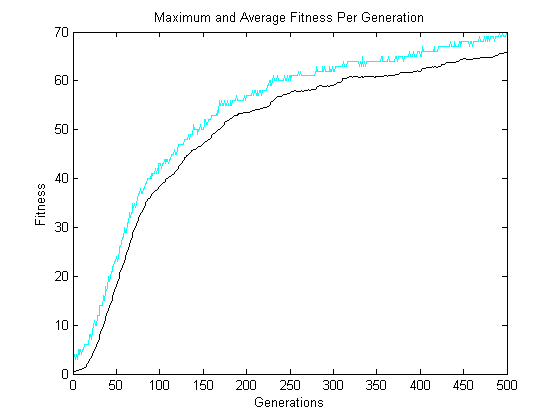
\includegraphics[scale=0.4]{fitnessfunction}
                \end{figure}
            \column{0.5\textwidth}
                Need a way to evaluate the population
        \end{columns}
    \end{frame}

    \begin{frame}{Fitness function}
        \begin{columns}
            \column{0.5\textwidth}
                \begin{figure}
                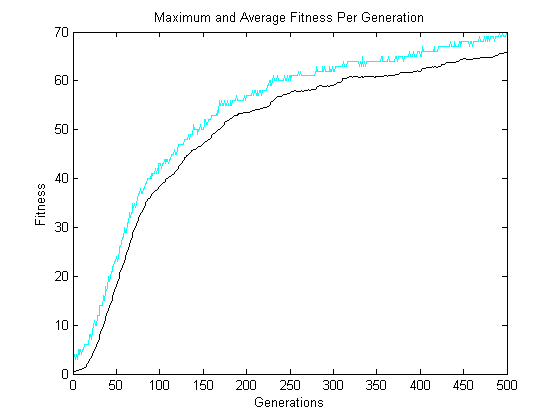
\includegraphics[scale=0.4]{fitnessfunction}
                \end{figure}
            \column{0.5\textwidth}
                \begin{figure}
                
\includegraphics[scale=0.04]{best}
                \end{figure}
        \end{columns}
    \end{frame}

    \begin{frame}{Fitness function}
        \begin{columns}
            \column{0.5\textwidth}
            \column{0.5\textwidth}
                \begin{figure}
                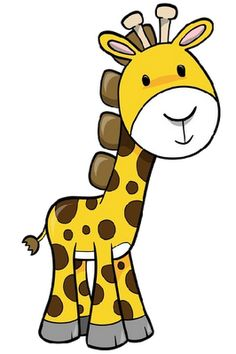
\includegraphics[scale=0.5]{giraffe}
                \end{figure}
        \end{columns}
    \end{frame}

    \begin{frame}{Fitness function}
        \begin{columns}
            \column{0.5\textwidth}
                int array - [Neck, foot size, length of tail]
            \column{0.5\textwidth}
                \begin{figure}
                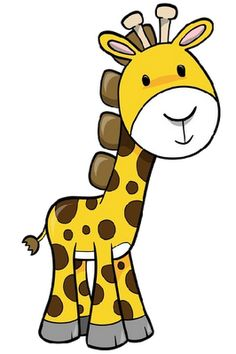
\includegraphics[scale=0.5]{giraffe}
                \end{figure}
        \end{columns}
    \end{frame}

    \begin{centering}
        \begin{frame}[c]{}
            \frametitle{Section 3}
            Selection
        \end{frame}
    \end{centering}

    \begin{frame}{Selection}
        \begin{columns}
            \column{0.5\textwidth}
                \begin{figure}
                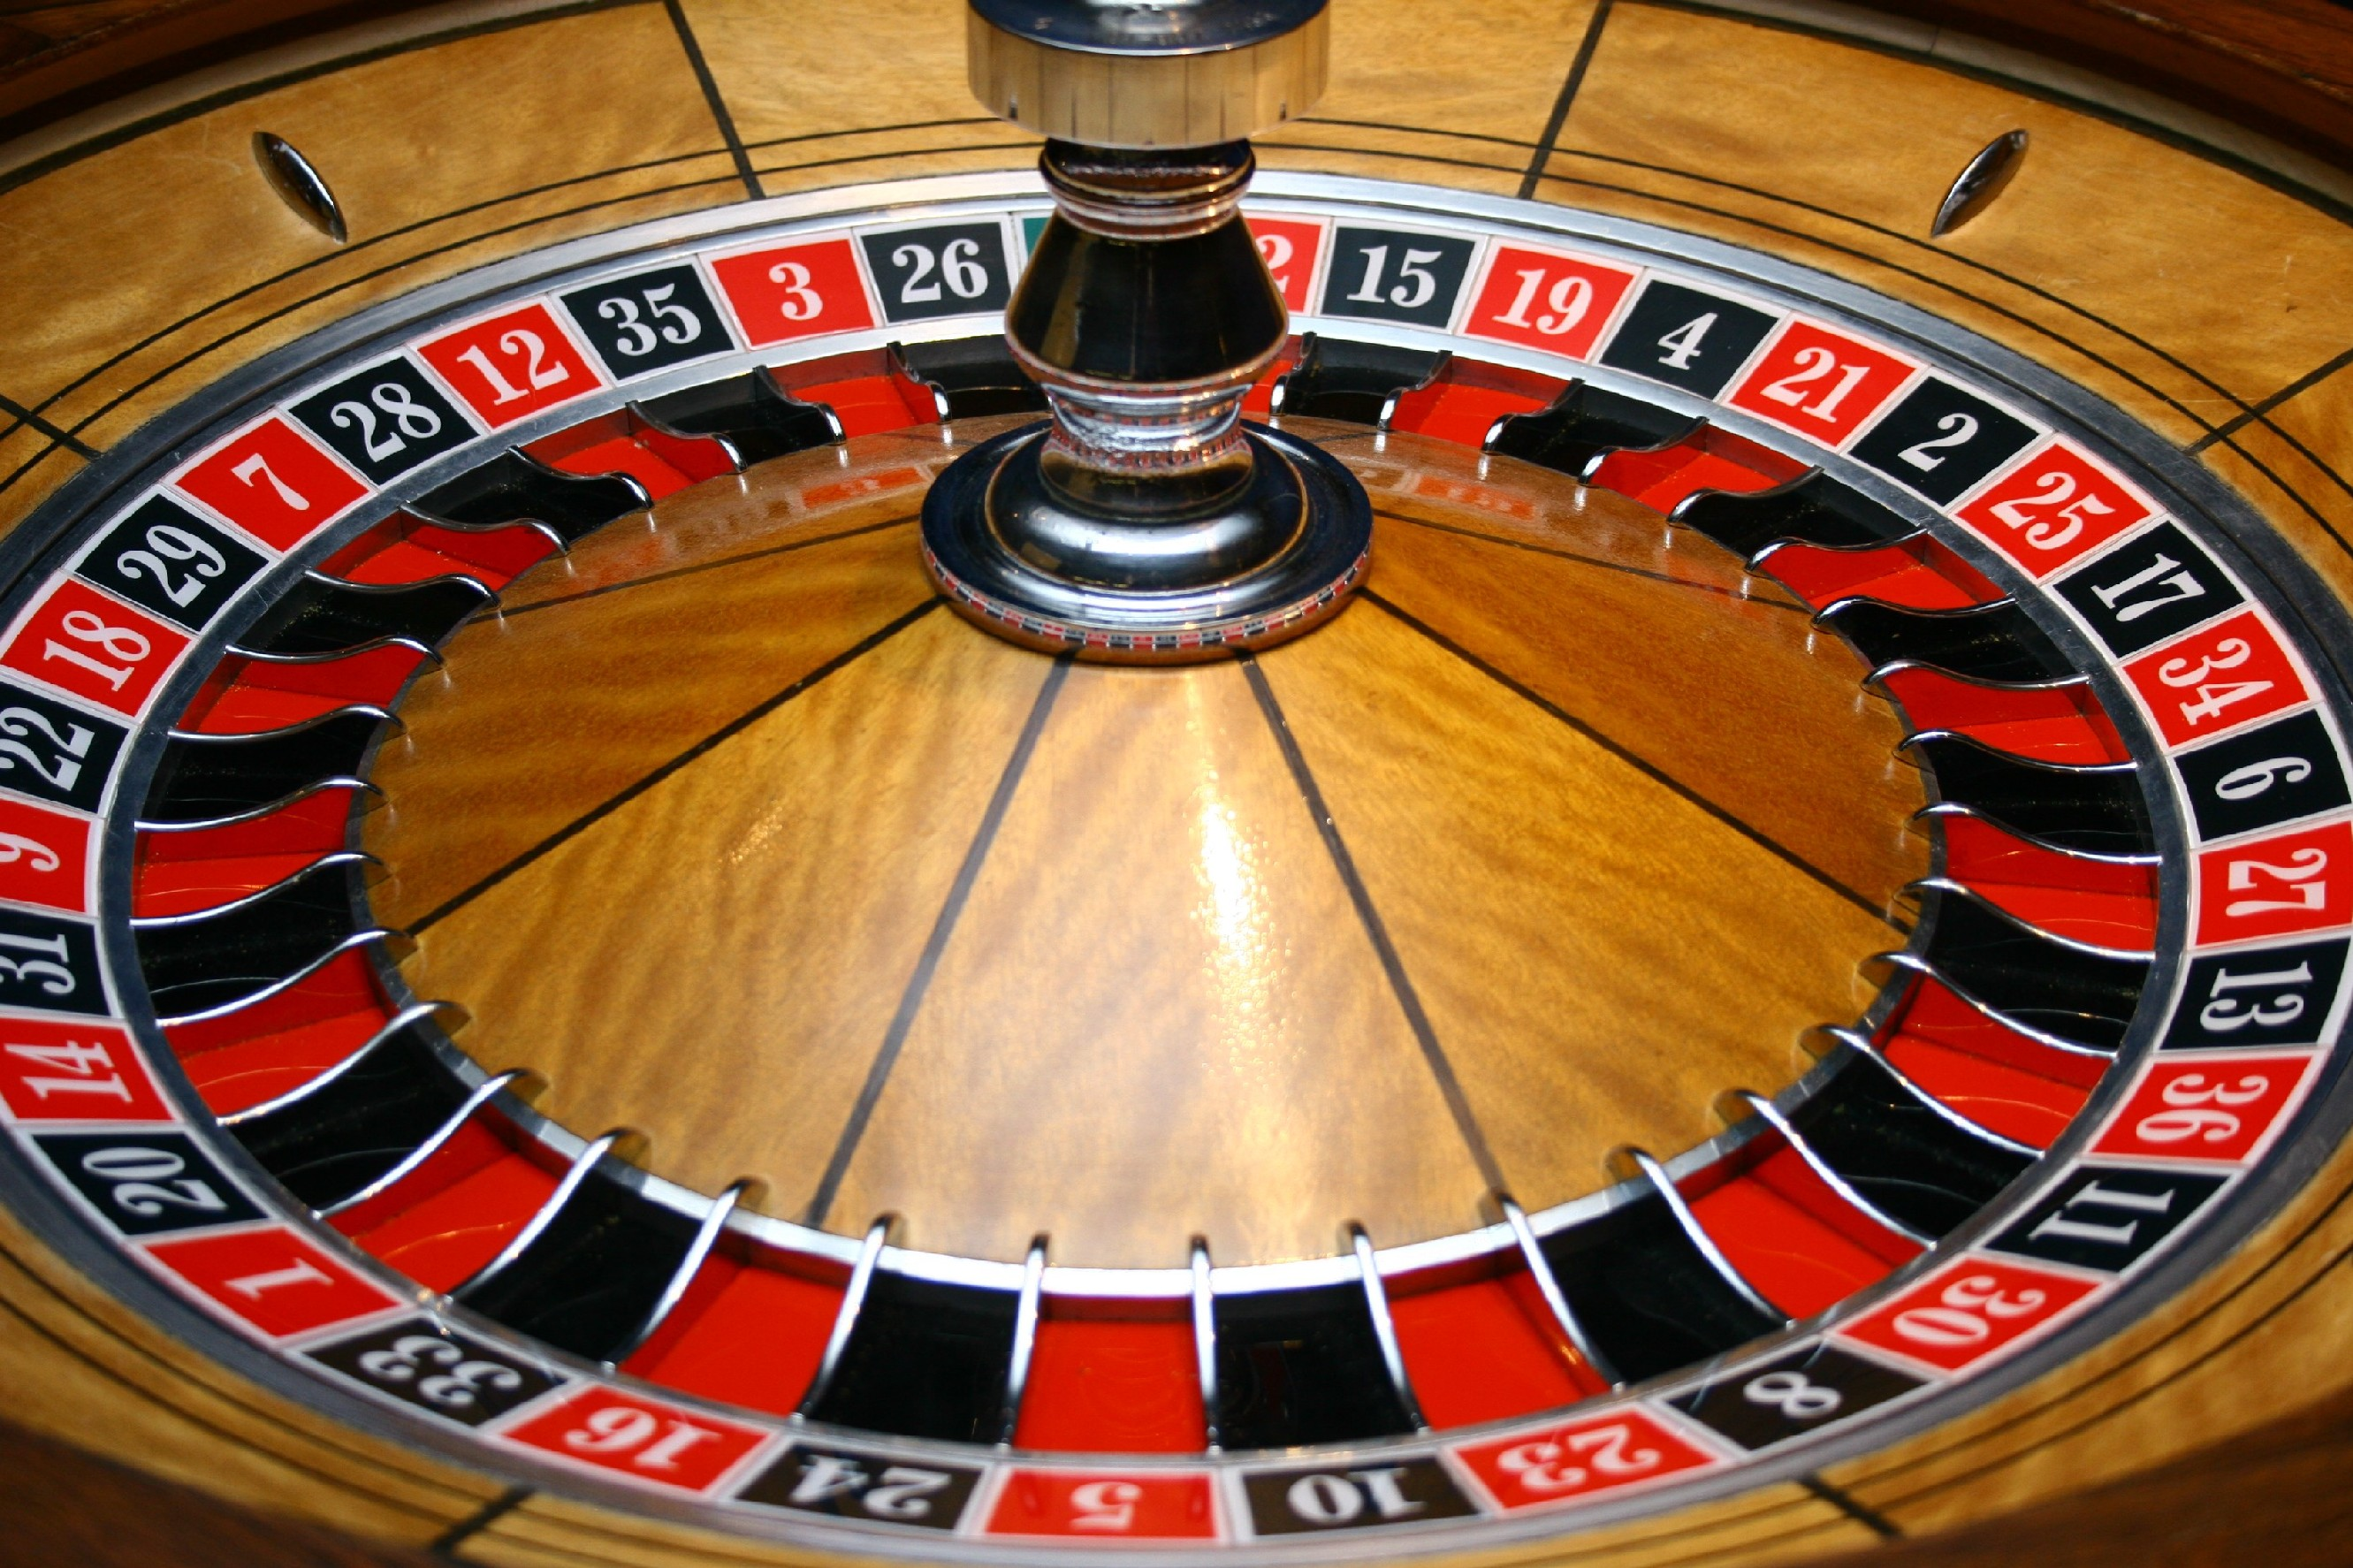
\includegraphics[scale=0.25]{roulette}
                \end{figure}
            \column{0.5\textwidth}
                Each chromosome gets a $ \frac{1}{n} $ chance\\
                But better ones get a bigger probability
        \end{columns}
    \end{frame}

    \begin{frame}{Selection}
        \begin{columns}
            \column{0.25\textwidth}
                Random
            \column{0.75\textwidth}
                \begin{figure}
                
\includegraphics[scale=0.4]{random}
                \end{figure}
        \end{columns}
    \end{frame}

    \begin{frame}{Selection}
        \begin{columns}
            \column{0.5\textwidth}
                \begin{figure}
                
\includegraphics[scale=0.145]{top10}
                \end{figure}
            \column{0.5\textwidth}
                The best of the best
        \end{columns}
    \end{frame}

    \begin{centering}
        \begin{frame}[c]{}
            \frametitle{Section 4}
            Heuristics
        \end{frame}
    \end{centering}

    \begin{frame}{Heuristics}
        \begin{columns}
            \column{0.5\textwidth}
                \begin{figure}
                
\includegraphics[scale=0.3]{thumb}
                \end{figure}
            \pause
            \column{0.5\textwidth}
                \begin{figure}
                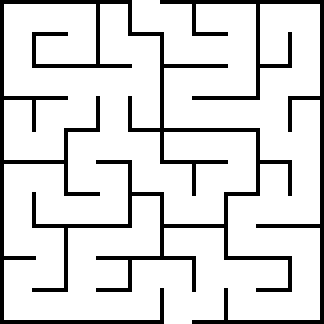
\includegraphics[scale=0.4]{maze}
                \end{figure}
        \end{columns}
    \end{frame}

    \begin{frame}{Crossover}
        \begin{columns}
            \column{0.5\textwidth}
                \begin{figure}
                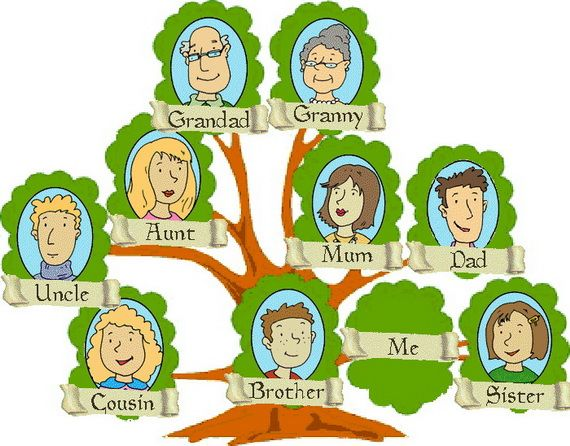
\includegraphics[scale=0.3]{family}
                \end{figure}
            \column{0.3\textwidth}
                One point\\
                Two point\\
                K point\\
                Uniform
        \end{columns}
    \end{frame}

    \begin{frame}{Ruin and recreate}
        \begin{columns}
            \column{0.5\textwidth}
                Destroy a section and rebuild
            \column{0.5\textwidth}
                \begin{figure}
                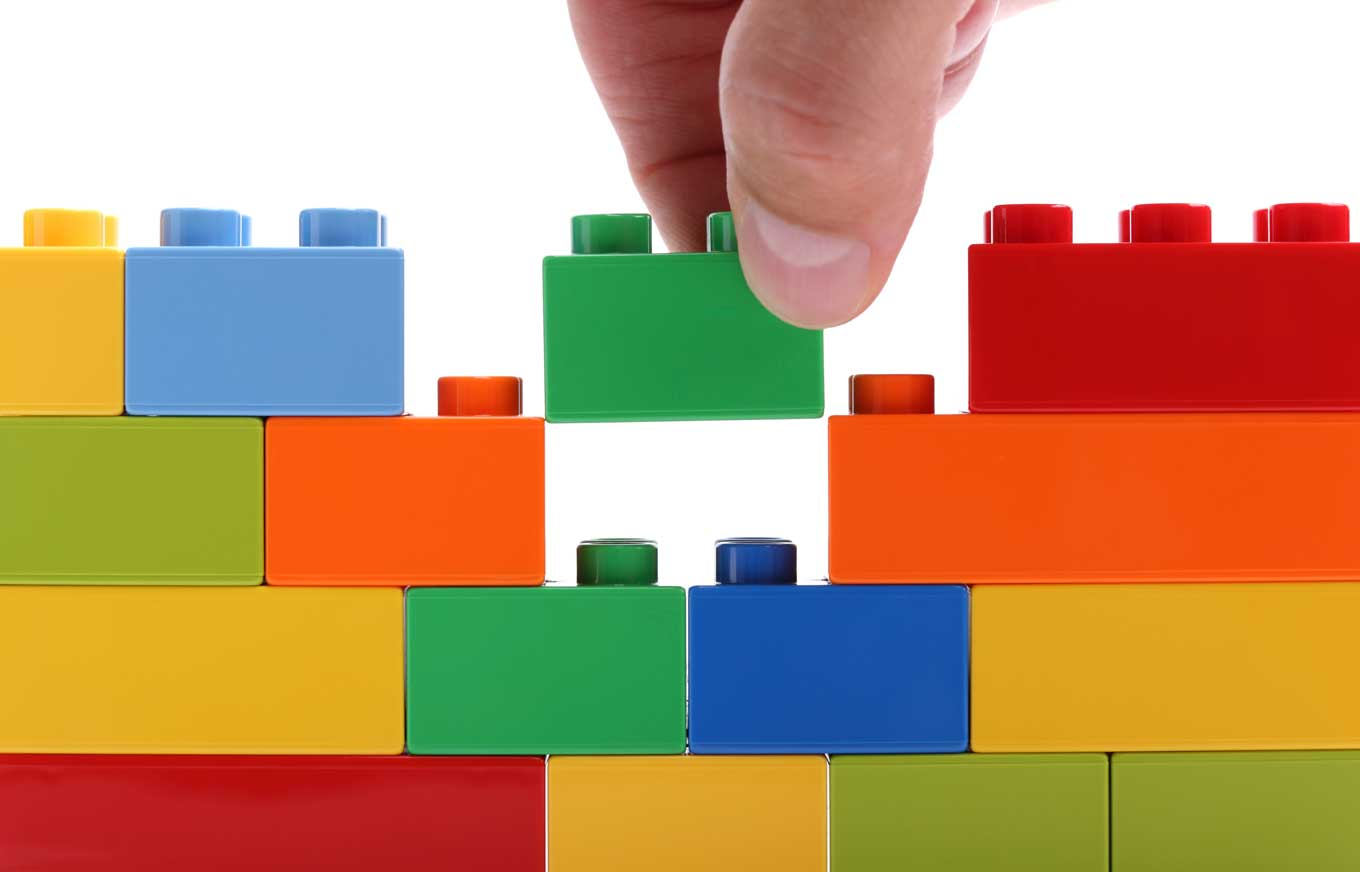
\includegraphics[scale=0.1]{rebuild}
                \end{figure}
        \end{columns}
    \end{frame}

    \begin{frame}{Mutation}
        \begin{columns}
            \column{0.5\textwidth}
                \begin{figure}
                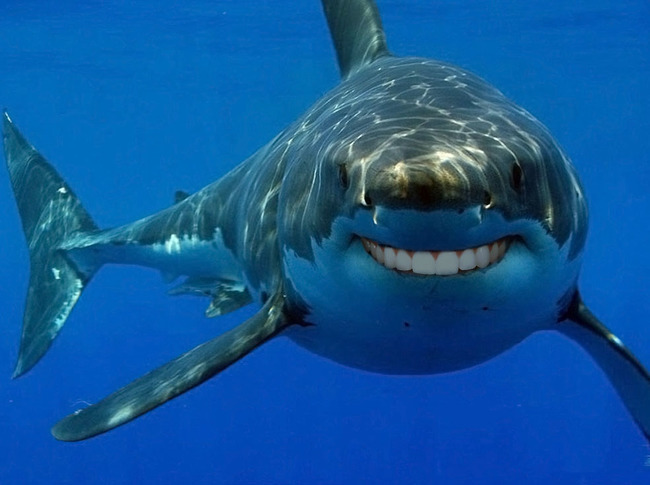
\includegraphics[scale=0.3]{shark}
                \end{figure}
            \column{0.2\textwidth}
                Mutants
        \end{columns}
    \end{frame}

    \begin{centering}
        \begin{frame}[c]{}
            \frametitle{Section 5}
            Killing the weakest
        \end{frame}
    \end{centering}

    \begin{frame}{Culling}
        \begin{columns}
            \column{0.5\textwidth}
                Keep the best
            \column{0.5\textwidth}
                \begin{figure}
                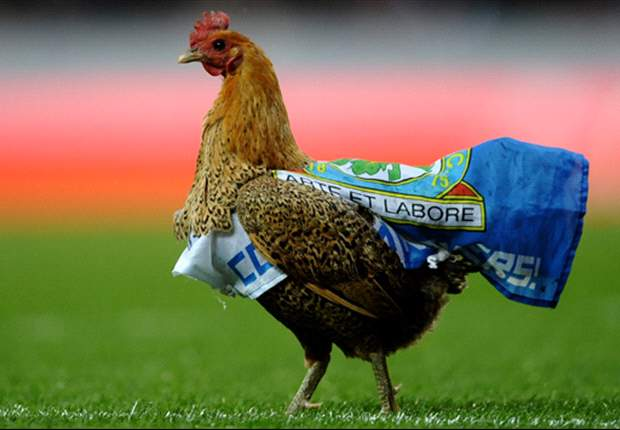
\includegraphics[scale=1]{chicken}
                \end{figure}
        \end{columns}
    \end{frame}

    \begin{centering}
        \begin{frame}[c]{}
            \frametitle{Section 6}
            Goals
        \end{frame}
    \end{centering}

    \begin{frame}{Average Fitness}
        \begin{columns}
            \column{0.5\textwidth}
                Repeat until the average is a set amount
            \column{0.5\textwidth}
                \begin{figure}
                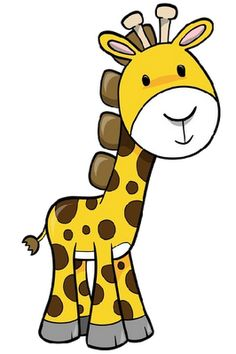
\includegraphics[scale=0.2]{giraffe}
                \caption{Steve}
                \end{figure}
        \end{columns}
    \end{frame}

    \begin{frame}{Average Fitness}
        \begin{columns}
            \column{0.5\textwidth}
                Repeat until the average is a set amount
            \column{0.5\textwidth}
                \begin{figure}
                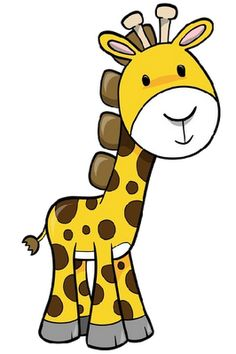
\includegraphics[scale=0.4]{giraffe}
                \caption{Dave}
                \end{figure}
        \end{columns}
    \end{frame}

    \begin{frame}{Generations}
        \begin{columns}
            \column{0.5\textwidth}
                \begin{figure}
                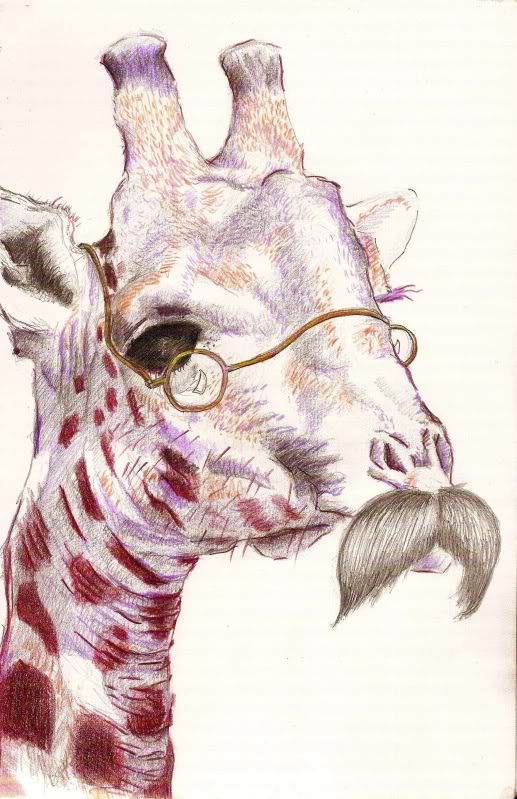
\includegraphics[scale=0.2]{OldGiraffe}
                \caption{Steve}
                \end{figure}
            \column{0.5\textwidth}
                Repeat until Steve gets old
        \end{columns}
    \end{frame}

    \begin{centering}
        \begin{frame}[c]{}
            \frametitle{Section 8}
            Problems
        \end{frame}
    \end{centering}

    \begin{frame}{Problems}
        \begin{enumerate}
            \item Chromosomal representation
            \item Local Maxima
            \item Heuristics are good
        \end{enumerate}
    \end{frame}

    \begin{centering}
        \begin{frame}[c]{}
            \frametitle{Section 8}
            But, why?
        \end{frame}
    \end{centering}

    \begin{frame}{Delilah}
        \begin{enumerate}
            \item Good
            \pause
            \item Scalable
            \pause
            \item Abstraction
        \end{enumerate}
    \end{frame}

    \begin{centering}
        \begin{frame}[c]{}
            \frametitle{That's all folks}
            Questions?
        \end{frame}
    \end{centering}

\end{document}
